\label{sec:evaluation}

This section answers the following questions:
\begin{itemize}
\item
  How effective is \Predator{} at detecting and predicting false sharing ($\S$~\ref{sec:effective})?

\item
  What is \Predator{}'s overhead, in terms of execution time ($\S$~\ref{sec:perfoverhead}) and memory ($\S$~\ref{sec:memoverhead})?

\item 
  How sensitive is \Predator{} to different sampling rates ($\S$~\ref{sec:sensitivity})? 
 
\end{itemize}

\paragraph{Experimental Platform.} All evaluations are performed on a quiescent Intel Core 2 dual-processor system equipped with 
16GB RAM. Each processor is a 4-core 64-bit Intel Xeon running at 2.33 GHz, with a 4MB shared L2 cache and 32KB private L1 cache. The underlying operating system is an unmodified CentOS 5.5, running with Linux kernel version 2.6.18-194.17.1.el5. We use glibc version 2.5 and LLVM version 3.2. 
All applications were compiled as 64-bit executables with the optimization level set to \texttt{-O1} in order to maintain accurate source code line number information.

\paragraph{Evaluated Applications.} 
This paper evaluates two popular benchmark suites,
Phoenix (with large input)~\cite{phoenix-hpca} and PARSEC (with simlarge input)~\cite{parsec}. We were unable to include two of the benchmarks. LLVM does not compile Facesim successfully, reporting an undefined template. Canneal compiles but then aborts unexpectedly. In addition to these benchmark suites, 
we evaluate \Predator{} on six real applications: MySQL, Boost, Memcached, aget, pbzip2 and pfscan.


\subsection{Detection and Prediction Effectiveness}
\label{sec:effective}

For every detected or predicted false sharing problem, \Predator{} reports source code information and detailed memory access information. Figure~\ref{fig:lrreport} shows an example for the linear\_regression benchmark. This report shows that the heap object starting with $0x40000038$ potentially causes numerous cache invalidations. The allocation callsite is provided to help locate culprits. In addition, \Predator{} also reports word-level access information of this object, which makes it possible for the developer to identify where and how false sharing occurs. From this information, we can see that this instance is a latent false sharing problem predicted by \Predator{}, since different threads are accessing different hardware cache lines. 

\begin{figure*}[!ht]
{\centering
\subfigure{\lstinputlisting[numbers=none,frame=none,boxpos=t]{fig/linearregression.report}}
\caption{False sharing report for the linear\_regression benchmark.
\label{fig:lrreport}}
}
\end{figure*}

\subsubsection{Benchmarks}
\label{sec:benchmarks}

\begin{table*}[ht!]
{\centering\begin{tabular}{l|r|r|r|r|r}\hline
{\bf \small Benchmark} & {\bf \small Source Code} & {\bf \small New} & {\bf \small Without Prediction} &{\bf \small With Prediction} & {\bf \small Improvement} \\
\hline
\small \textbf{histogram} & {\small histogram-pthread.c:213} & \cmark{} &\cmark{} & \cmark{} & 46.22\%\\
\small \textbf{linear\_regression} & {\small linear\_regression-pthread.c:133} & & & \cmark{} & 1206.93\% \\
\small \textbf{reverse\_index} & {\small reverseindex-pthread.c:511} & & \cmark{} & \cmark{} & 0.09\%\\
\small \textbf{word\_count} & {\small word\_count-pthread.c:136} & & \cmark{} & \cmark{} & 0.14\%\\
\hline
\small \textbf{streamcluster} & {\small streamcluster.cpp:985} &  & \cmark{} & \cmark{} &7.52\% \\
\small \textbf{streamcluster} & {\small streamcluster.cpp:1907} & \cmark{} & \cmark{} & \cmark{} & 4.77\%\\
\hline
\end{tabular}
\caption{False sharing problems in the Phoenix and PARSEC benchmark suites. \label{table:detection}}
}
\end{table*}

Table~\ref{table:detection} provides detection results across the Phoenix and PARSEC benchmark suites. 
The first column lists the programs with false sharing problems.  The second column shows precisely where the problem is. Because all discovered false sharing occurs inside heap objects, we present callsite source code information here.  The third column, \emph{New}, indicates whether this false sharing was newly discovered by \Predator{}.  A checkmark in the following two columns indicates whether the false sharing was identified without
prediction and/or with prediction.  The final column, \emph{Improvement}, presents the performance improvement after fixing false sharing.

As the table shows, \Predator{} reveals two previously unknown false sharing problems. It is the first tool to detect false sharing problems in histogram and in line $1908$ of streamcluster. 
In histogram, multiple threads simultaneously modify different locations of the same heap object, thread\_arg\_t. 
Padding this data structure eliminates false sharing and improves performance by around 46\%. In streamcluster, multiple threads simultaneously access and update the same \texttt{bool} array, switch\_membership. Simply changing all elements of this array to a \texttt{long} type reduces the false sharing and improves performance by about 4.7\%.

%, although it is not a complete fix of false sharing. 
%None of these two false sharing problems has been reported by previous tools.
Other false sharing problems reported here were also discovered by previous work~\cite{sheriff}. We do not see significant performance improvement for the reverse\_index and word\_count benchmarks. They are reported here because the number of cache invalidations in these two programs crosses our predefined threshold.
Increasing \Predator{}'s reporting threshold would avoid reporting these cases, which are relatively insignificant.
Nonetheless, it is worth noting that these two benchmarks do indeed have false sharing problems,
which can be confirmed by the word-level information generated by \Predator{}. 

The streamcluster benchmark has another false sharing problem located at line $985$. Different threads repeatedly update the work\_mem object. The authors of streamcluster were clearly aware of this issue and provide a CACHE\_LINE macro for padding. Unfortunately, the default value of this macro is set to $32$ bytes, which is smaller than the actual cache line size of the experimental machine. Setting it to $64$ bytes instead improves performance by about 7.5\%.

The linear\_regression benchmark has an unusually severe false sharing problem. Fixing it improves performance by more than $12\times$. In this benchmark, different threads repeatedly update their thread-specific locations inside the tid\_args object inside a tight loop. Interestingly, Nanavati et al. observe that this false sharing problem occurs when using clang and disappears when using gcc with the \texttt{-O2} and \texttt{-O3} optimization levels~\cite{OSdetection}. However, we observe a different result when using our version of clang and the custom memory allocator: the false sharing problem \emph{does not occur at all} because the offset of the starting address of the potentially falsely-shared object and the start of cache line is 56 bytes (see Figure~\ref{fig:perfsensitive}). As we discuss below,\Predator{}'s prediction mechanism identifies this latent false sharing problem, highlighting the value of predictive detection.

\subsubsection{Real Applications}
To verify \Predator{}'s utility, we evaluate its effectiveness on several widely-used real applications. These applications include a database server (MySQL~\cite{mysql}),
a standard C++ library (Boost~\cite{libfalsesharing}),
a distributed memory object caching system (Memcached), a download accelerator (aget),
a parallel bzip2 file compressor (pbzip2), and a parallel file scanner (pfscan).

MySQL-5.5.32 and boost-1.49.0 are known to have false sharing problems. The other applications we examine (memcached-1.4.15, aget-0.4.1 and pbzip2-1.1.6) do not have  any known false sharing problems.

MySQL's false sharing problem caused a significant scalability problem and was very difficult to identify.
According to the architect of MySQL, Mikael Ronstrom, ``we had gathered specialists on InnoDB..., participants from MySQL support... and a number of generic specialists on 
computer performance...'', ``[we] were able to improve MySQL performance by 6$\times$ with those scalability fixes''~\cite{mysql}. 
The false sharing inside Boost is caused by the usage of a spinlock pool. Different threads may utilize different spinlocks located in the same cache line in this case. Fixing it brings a 40\% performance improvement.
\Predator{} is able to pinpoint the false sharing locations in both MySQL and the Boost library. 
For the other four applications, \Predator{} does not identify any severe false sharing problems.

\subsubsection{Prediction Effectiveness}
\label{sec:predicteval}
In this section, we describe in detail our experience with a particular benchmark that demonstrates the value of our approach. We use the linear\_regression benchmark as a case study for the following reasons: (1) the false sharing problem of this benchmark cannot be detected without prediction; (2) false sharing severely degrades performance when it actually occurs. Hence, it is a serious problem that should always be detected. 

\begin{figure}[!t]
{\centering
\subfigure{\lstinputlisting[numbers=none,frame=none,boxpos=t]{fig/linearregression.psedocode}}
\caption{The false sharing problem inside the linear\_regression benchmark.
\label{fig:linearregression}}
}
\end{figure}

Figure~\ref{fig:linearregression} shows the data structure and the source code experiencing false sharing. The size of this data structure, lreg\_args, is $64$ bytes 
when the program is compiled to a $64$-bit binary. For this benchmark, the main thread allocates an array containing as many elements as the number of underlying hardware cores. Each element is a lreg\_args type with $64$ bytes. This array is then passed to different threads (lreg\_thread function) so that each thread only updates its thread-dependent area. False sharing occurs if two threads happen to update data in the same cache line. 

Figure~\ref{fig:perfsensitive} shows how sensitive linear\_regression's performance is to different starting addresses of a falsely-shared object. When the offset is $0$ or $56$ bytes, this benchmark achieves its optimal performance and has no false sharing. When the offset is $24$ bytes, the benchmark runs around $15\times$ slower because of false sharing.

\subsection{Performance Overhead}
\label{sec:perfoverhead}

\begin{figure*}[!t]
\begin{center}
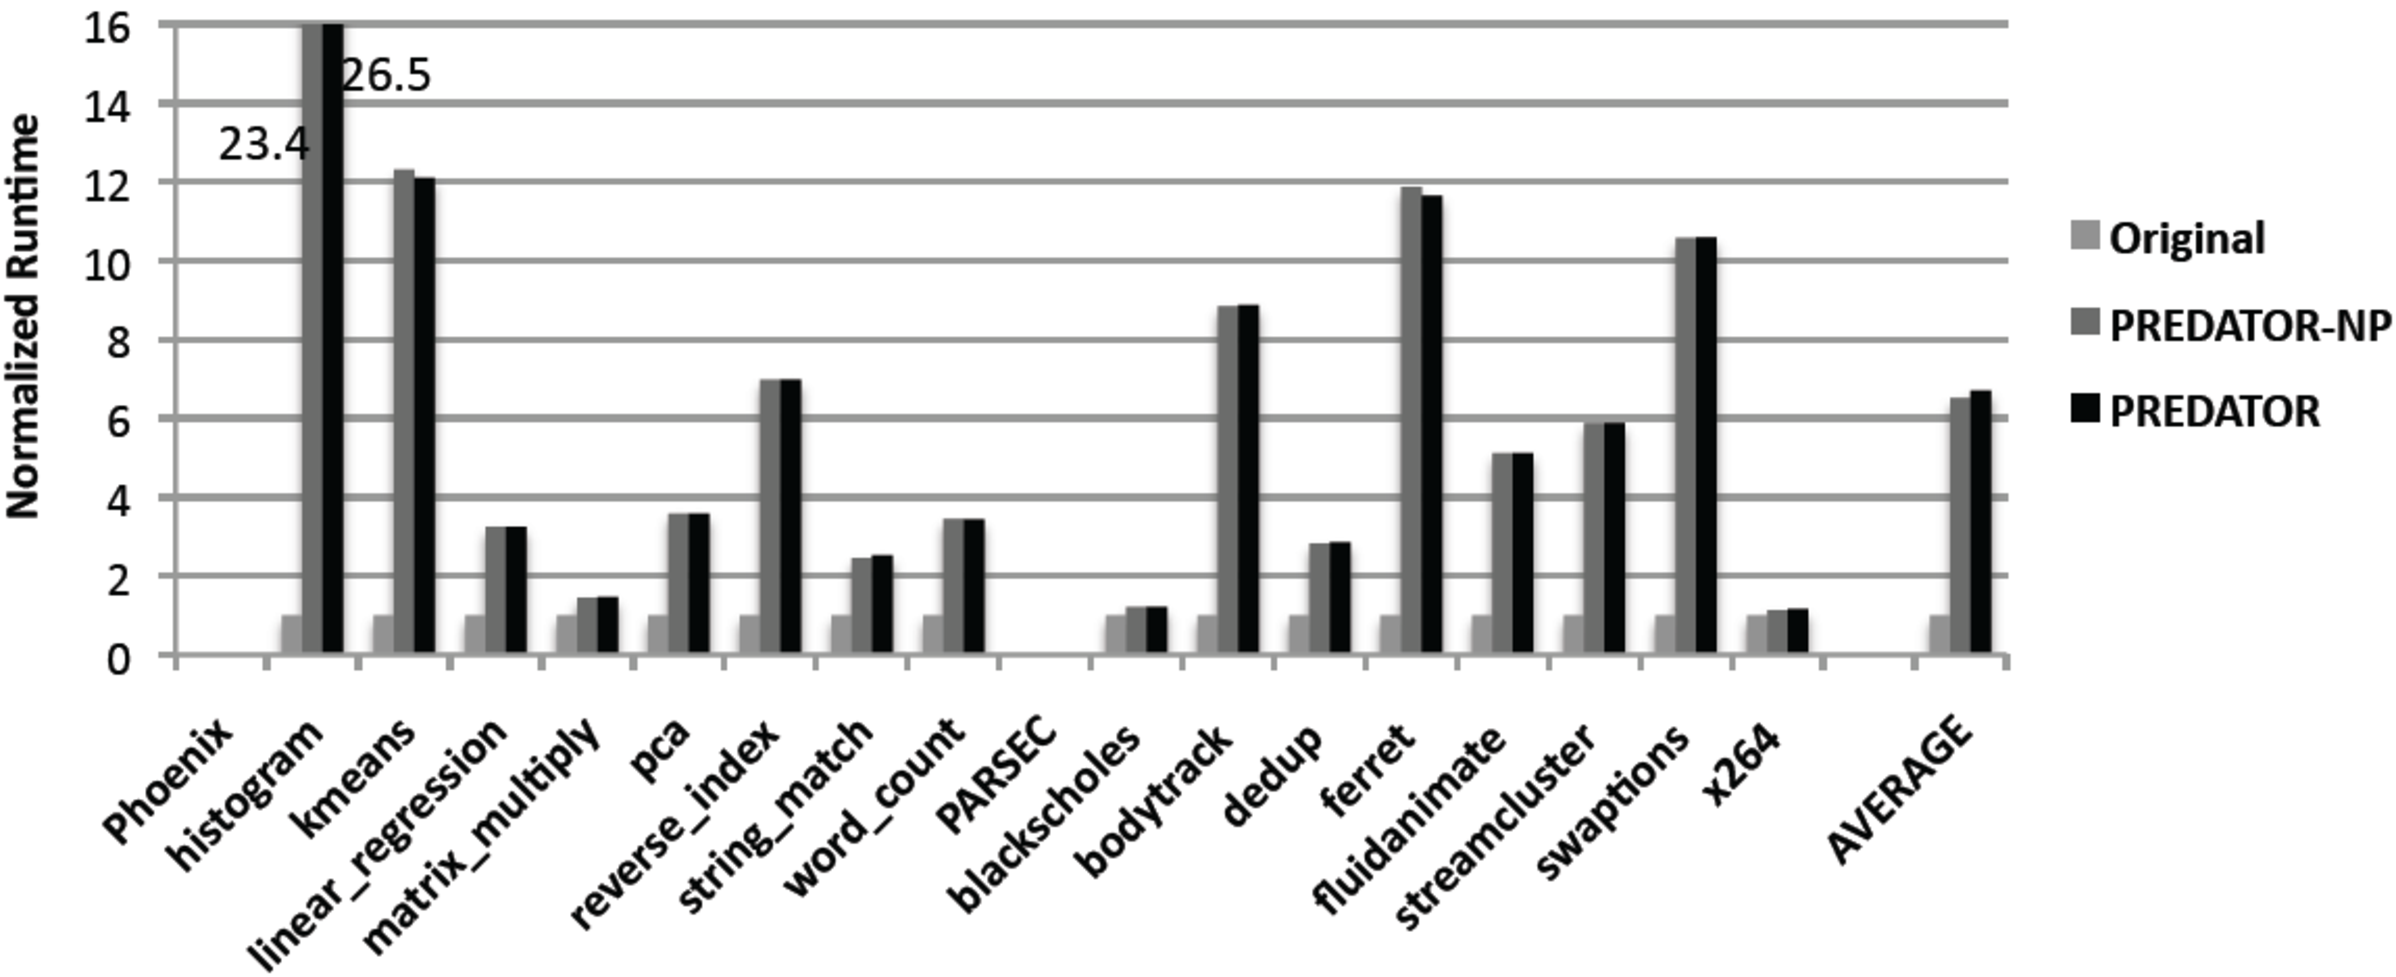
\includegraphics[width=6.5in]{fig/perf}
\end{center}
\caption{
Performance overhead of \Predator{} with and without prediction (PREDATOR-NP).
\label{fig:perf}}
\end{figure*}


Figure~\ref{fig:perf} presents runtime overhead for using \Predator{}. All 
measurements are based on the average of $10$ runs, excluding the maximum and minimum values. Overall, \Predator{} imposes an average of $5.4\times$ performance overhead. There is no noticeable difference on performance whether the prediction mechanism is enabled or not. 
 
Five of these (histogram, kmeans, bodytrack, ferret, and swaptions), have more than $8\times$ performance overhead. The histogram benchmark runs more than $26\times$ slower because tracking detailed accesses to cache lines with false sharing exacerbates the false sharing effect (see Section~\ref{sec:sample}). Although bodytrack and ferret have no false sharing, \Predator{} detects numerous cache lines with writes that exceed the {\it TrackingThreshold}, causing it to track detailed access information. We have not identified the exact cause of \Predator{}'s high performance overhead for kmeans.
   
As expected, \Predator{} imposes relatively little overhead for I/O-bound applications (matrix\_multiply, blackscholes, x264, aget, Memcached, pbzip2, and pfscan).

\subsection{Memory Overhead}
\label{sec:memoverhead}

Figure~\ref{fig:memusage} presents \Predator{}'s memory overhead. We account for \Predator{}'s physical memory consumption by collecting information on the proportional set size (PSS) in \texttt{/proc/self/smaps}, which reflects the physical memory increase on the existing system of running an application~\cite{memusage}. We periodically collect this data and use the sum of different memory mappings as the total physical memory usage of running an application.

\Predator{} imposes less than 50\% memory overhead for 17 out of 22 applications.  For swaptions and aget, \Predator{} introduces high \emph{relative} memory overhead because their original memory footprints are extraordinarily small (only $3$ kilobytes). We are continuing to investigate the source of MySQL's large increase in memory consumption (from 132MB to 1.3GB). Nonetheless, even in the cases when \Predator{}'s absolute memory overhead is high, all of these applications comfortably fit into RAM on modern platforms.

\begin{figure*}[!t]
\begin{center} 
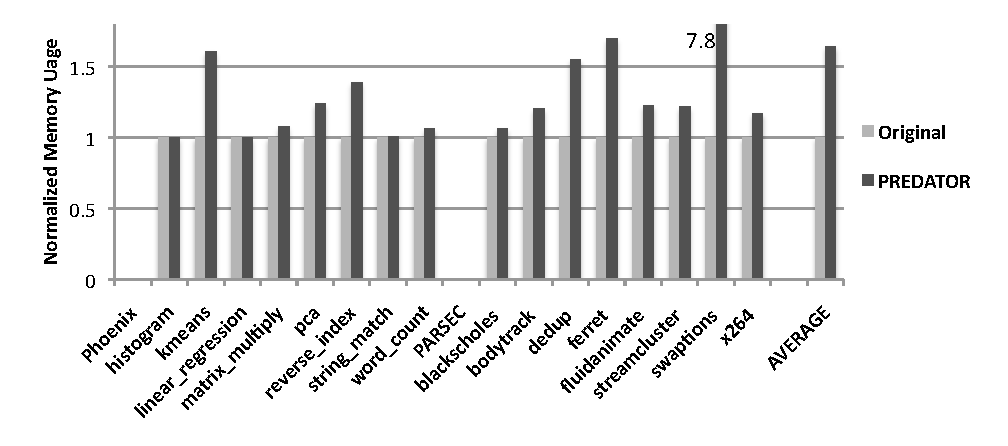
\includegraphics[width=6.5in]{fig/memusage}
\end{center}
%\includegraphics{fig/potential.pdf}
\caption{Normalized physical memory usage overhead with \Predator{}.}
\label{fig:memusage}
\end{figure*}


\subsection{Sensitivity to Different Sampling Rates}
\label{sec:sensitivity}

Section~\ref{sec:sample} describes \Predator{}'s sampling approach to reduce tracking overhead. This section evaluates the effect of different sampling rates on performance and effectiveness. Note that running an application with different sampling rates does not affect its memory usage.

The default sampling rate used by \Predator{} is 1\%. To test \Predator{}'s sensitivity to this choice, we evaluate performance on a representative subset of the benchmarks with two other sampling rates: 0.1\% and 10\%. Figure~\ref{fig:sample} presents the results. As expected, \Predator{} introduces lower performance overhead at lower sampling rates. Even when using the 0.1\% sampling rate, \Predator{} is still able to detect all false sharing problems reported here, although it reports a lower number of cache invalidations.
 
\begin{figure}[!t]
\begin{center} 
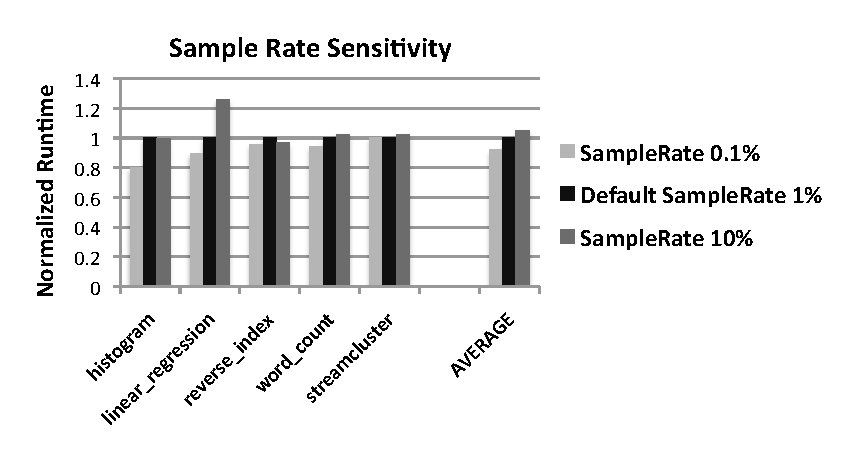
\includegraphics[width=3.4in]{fig/sample}
\end{center}
%\includegraphics{fig/potential.pdf}
\caption{Normalized execution time for different sampling rates.}
\label{fig:sample}
\end{figure}


